\documentclass[aspectratio=169]{beamer}

\usetheme{vega}

\title{Report on my research}
\subtitle{SRG Market microstructure}
\author{Vsevolod Zaostrovsky}
\institute{Vega Institute Foundation}
\supervisor{Anton Belyakov, Alexey Savin}
% \date{August 21 -- 28, 2022}

\usepackage[]{lipsum}
\begin{document}
\maketitle

\begin{frame}{Data specification}
    \begin{figure}
        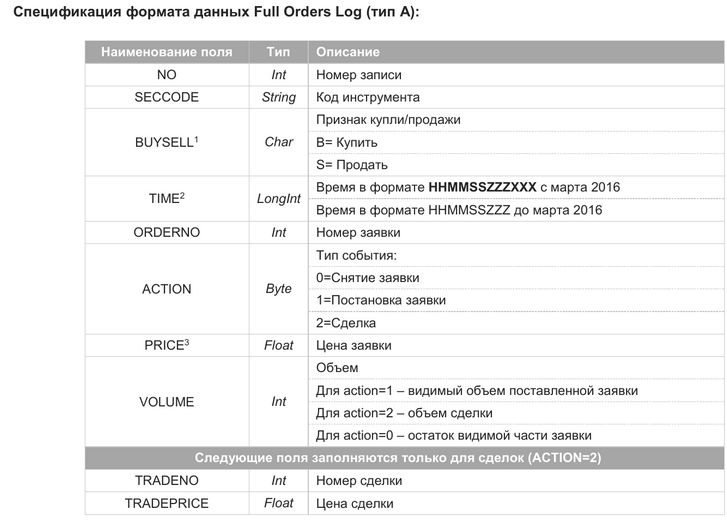
\includegraphics[scale=0.55]{figs/spec.png}
        \caption{Specification}
        \label{fig:mvslim}
    \end{figure}
\end{frame}

\begin{frame}{Data preparing --- 1}
        Initially, the parser data was in the form of:
        \begin{equation*}
            [[ 102.260, 50 ], [ 102.280, 100 ], [ 102.294, 35 ], [ 102.310, 200 ], [ 102.500, 2546 ], [0., 0.]]
        \end{equation*}
        I changed it to give the data in the following form:
        \begin{align*}
            & 10:00:01.000609985 \ [[ 61.782, 40000 ], [ 61.870, 100000 ], \cdots] \\
            & \textrm{Price } 61.79 \textrm{ Vol } 40000  \\
            & 10:00:01.000609985 \ [[ 61.870, 100000 ], \cdots]
        \end{align*}
        I choose all the deals and for each deal the parser prints the LOB before and after the deal
        and the price and volume of order in between.  
        Then using Python I collected vectors of four numbers: 
        (Time, AskBefore, AskAfter, Volume).
\end{frame}

\begin{frame}{Data preparing --- 2}
    % Then using Python I collected vectors of four numbers: (Time,AskBefore,AskAfter,Volume).
    \begin{figure}
        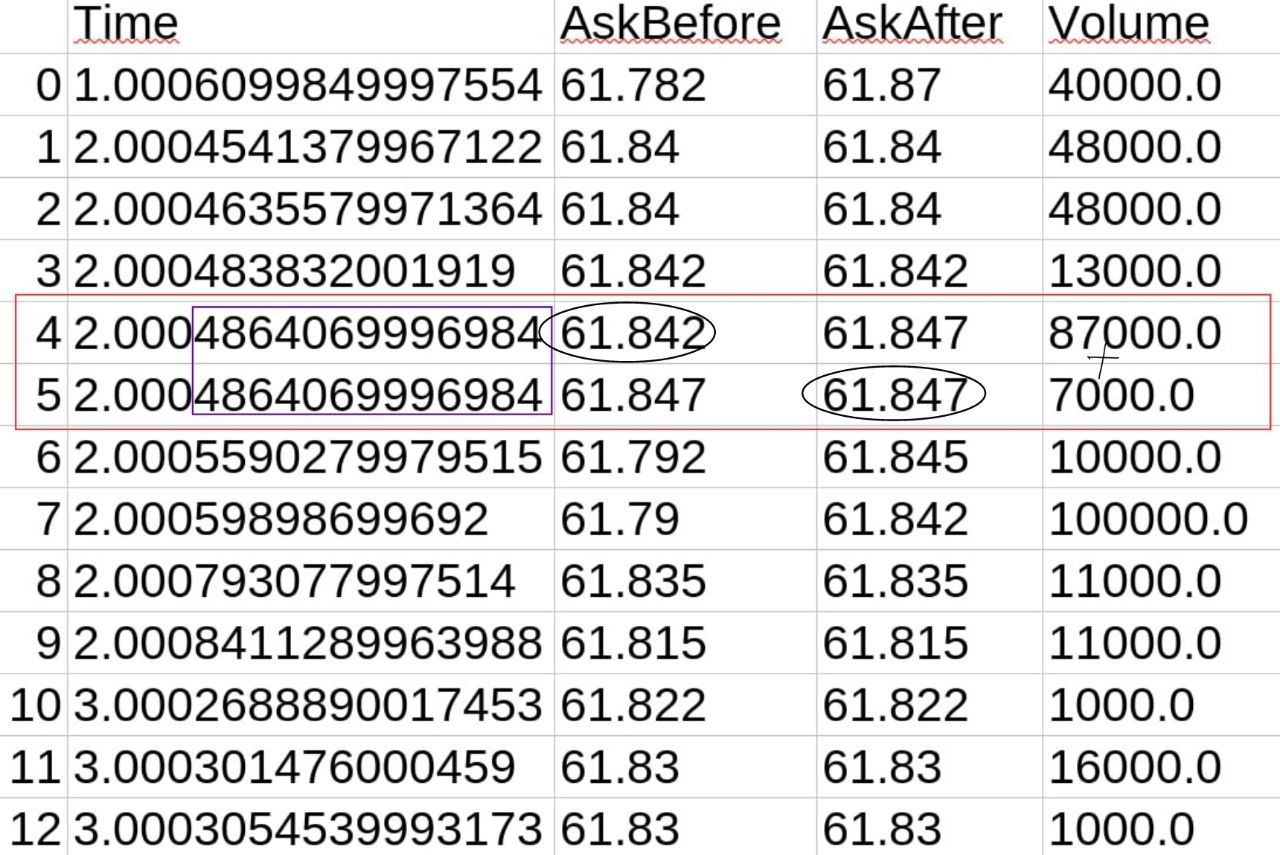
\includegraphics[scale=0.31]{figs/datscsv.jpg}
        \caption{Data in csv format}
        \label{fig:mvslim}
    \end{figure}
\end{frame}


\begin{frame}{Our methodology to fit parameters $\rho, \kappa, q$}
    We chose regression to find parameters:                                                                                                                                                                                                                                                                                                                                                                                       
            \begin{equation*}
                \frac{\Delta A_{k+2}}{\Delta t_{k+2}} - \frac{\Delta A_{k+1}}{\Delta t_{k+1}} 
        = - \rho \Delta A_{k+1} + \rho \lambda x_{k+1} + (\kappa + \lambda) (\frac{x_{k+2}}{\Delta t_{k+2}} - \frac{x_{k+1}}{\Delta t_{k+1}}).
            \end{equation*}

        Where all the information needed can be extracted from the l3 data: 
        \begin{itemize}
            \item $\Delta A_{k}$ is an ask change after execution of the limit order with the depth $x_k$.
            So, $\Delta A_{k} = \textrm{AskAfter}(k) - \textrm{AskBefore}(k)$ and $x_k = \textrm{Volume}(k)$.
            \item $\Delta t_{k}$ is a time between $k$ and $k + 1$ orders of dataset. So, $\Delta t_{k} = \textrm{Time}(k+1) - \textrm{Time}(k)$
        \end{itemize}
\end{frame}


\begin{frame}{Regression results -- all the data.}
    \begin{figure}
        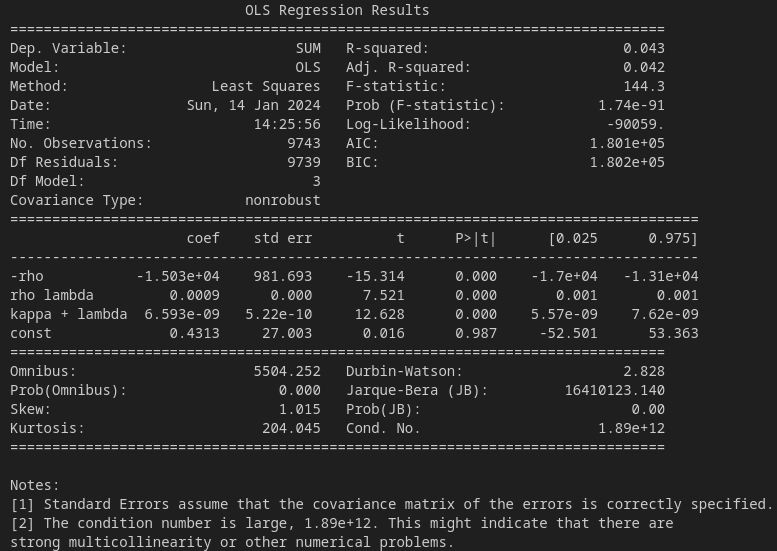
\includegraphics[scale=0.49]{figs/RegAD.png}
        \caption{All the data}
        \label{fig:mvslim}
    \end{figure}
\end{frame}

\begin{frame}{Regression results -- more then zero.}
    \begin{figure}
        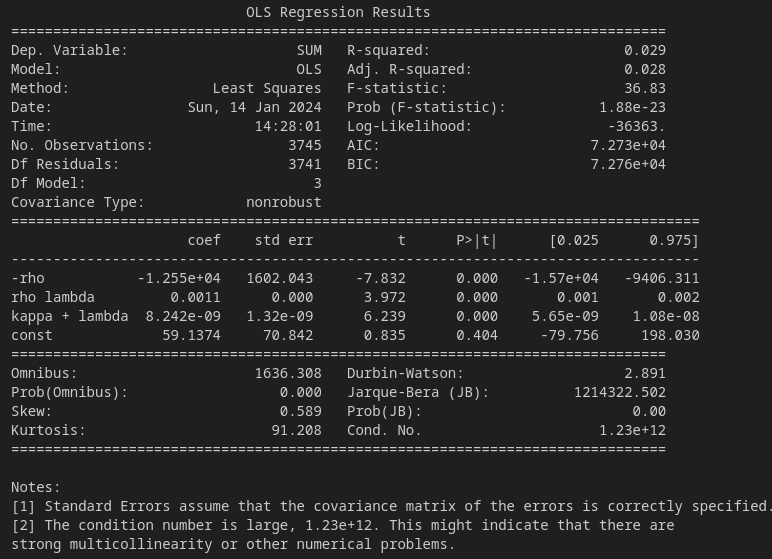
\includegraphics[scale=0.49]{figs/RegMZ.png}
        \caption{More then zero}
        \label{fig:mvslim}
    \end{figure}
\end{frame}

\begin{frame}{Regression results -- more then 100bp.}
    \begin{figure}
        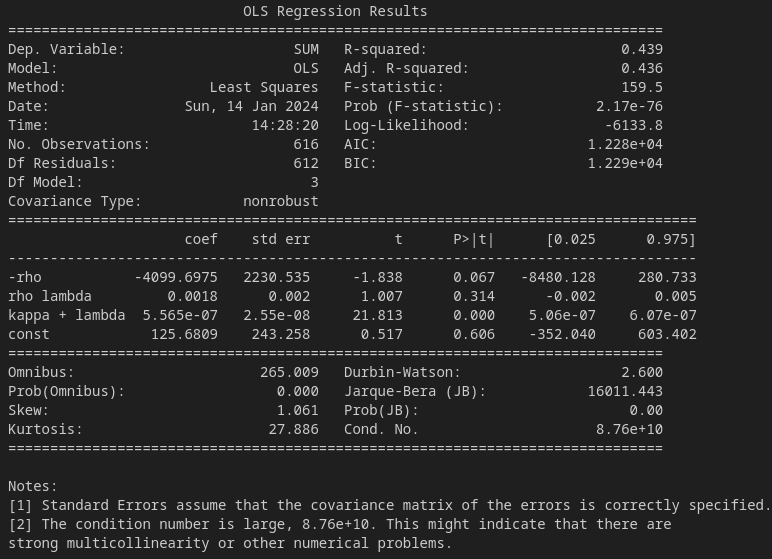
\includegraphics[scale=0.49]{figs/Reg100bp.png}
        \caption{More then 100bp}
        \label{fig:mvslim}
    \end{figure}
\end{frame}

\begin{frame}{Backtest procedure.}
    \begin{itemize}
        \item Find big gaps and remember next asks and deals for each.
        \item Consider big deal and little deals as ours and calculate metrics for them.
        \item Research if asks dynamics follows $A_t = \overline p _t + \frac{s}{2} + x_1 \kappa e^{- \rho t}$.
    \end{itemize}
    \begin{figure}
        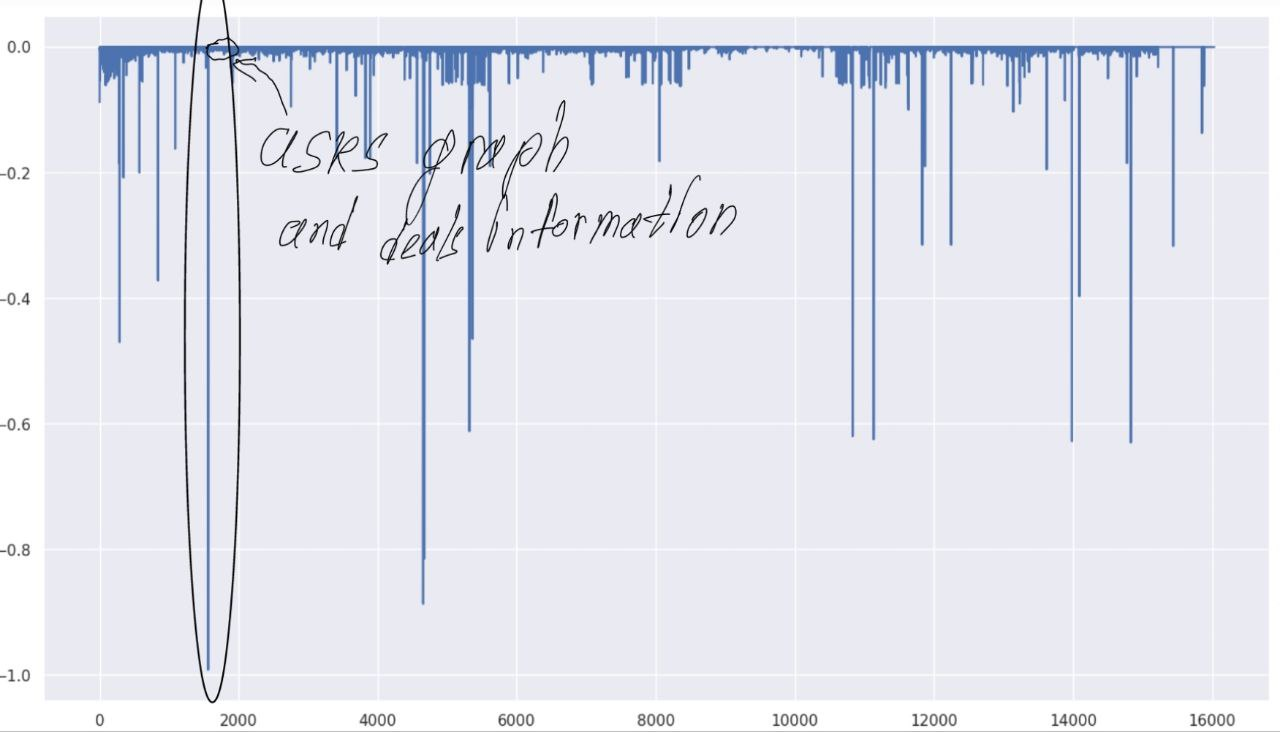
\includegraphics[scale=0.22]{figs/bt_met.jpg}
        \caption{Methodology}
        \label{fig:mvslim}
    \end{figure}
\end{frame}


\begin{frame}{Important (imho) Ideas and Questions}
    \begin{itemize}
        \item Backtest procedure... See the previous frame.
        \item It is interesting what is happening with other instruments. Also, the important idea: for some instruments OW model is useless. For which?
        \item It is interesting what is happening with that instrument throughout the day. We can consider structural breaks and fit the model on different sygments.
        \item What does mean regression results?
        \item Have I done everything right?
        \item What else can we do?
        \item Does my bt methodology correct?
    \end{itemize}
\end{frame}

\end{document}